\chapter{Overenie riešenia}

Keďže sme natrénovali viacero modelov, ako prvé sme vykonali ich porovnanie pomocou implementáciou metódy RISE pre 3D snímky.
Následne sme vybrali z nich najlepší model, ktorý sme používali v ďaľších experimentoch.

\paragraph{Adresovanie náhodnosti metódy RISE pri porovnávaní dvoch roznych modelov}

Keďže vygenerované masky sú náhodné, pri porovnávaní dvoch metód (kombinácii rôznych parametrov metódy RISEI) generujeme rovnaké binárne masky pre každý i-ty snímok, tj. zakryté pozície sú rovnaké, rôzna je len hodnota zakrytia. Vygenerované binárne masky pre jednotlivé snímky v testovacej sade sú stále náhodné (a teda aj medzi sebou rôzne). Rovnaké sú len binárne masky pre dve rôzne generovania masiek pre ten istý snímok v testovacej sade. Takto dosiahneme kvalitnejšie výsledky, pretože žiadna metóda nebude mať výhodu, že náhodou zakryla rôzne časti snímky lepšie a teda bude dôležité ako ich zakryla.

\section{Experimenty}

\subsection{Porovnanie metódy RISE na natrénovaných modeloch \label{sec:experiment_rise_various_architectures}}

V tomto experiemnte sme porovnali metódu RISE na nami natrénovaných modeloch. Vybrali sme najlepšie natrénované modely pre každú architektúru (Tabuľka \ref{tab:model_training_results}). Použili sme nami implementovaný metódu RISEI pričom sme nastavili jej parametre tak, aby fungovala ako metóda RISE.
Parametre sme nastavili nasledovne: $s = 8$, $p = 1/3$, $b1 = 0$, $b2 = 1$ (opis parametrov sa nachádza v tabuľke \ref{tab:risei_params}). Na vytvorenie tepelnej mapy sme vygenerovali 1024 masiek. Pri vyhodnocovaní metrík insertion a deletion sme nastavili veľkosť kroku na 2500 voxelov (takto trvalo vyhodnotenie tepelnej mapy ~3 minúty). Vybrali sme 25 náhodných snímkov z testovacej sady, generovanie a vyhodnotenie tepelných máp k nim trvalo približne ~1 hodinu. Najlepšie výsledky sme dosiahli na architektúre 3D CNN (Tabuľka \ref{tab:experiment_rise_various_architectures}).

\begin{table}[]
    \centering
    \begin{tabular}{cl|r|r|r|}
        \cline{3-5}
        \multicolumn{1}{l}{} &  & \multicolumn{1}{c|}{3D CNN} & \multicolumn{1}{c|}{3D ResNET} & \multicolumn{1}{c|}{2D ResNET} \\ \hline
        \multicolumn{1}{|c|}{\multirow{2}{*}{Insertion (AUC)}} & priemer & \textbf{0.50} & 0.46 & 0.38 \\ \cline{2-2}
        \multicolumn{1}{|c|}{}                                 & medián  & \textbf{0.53} & 0.13 & 0.30 \\ \cline{1-2}
        \multicolumn{1}{|c|}{\multirow{2}{*}{Deletion (AUC)}}  & priemer & \textbf{0.53} & 0.81 & 0.62 \\ \cline{2-2}
        \multicolumn{1}{|c|}{}                                 & medián  & 0.60 & 0.83 & \textbf{0.43} \\ \hline
    \end{tabular}
    \caption{\textbf{Porovnanie metódy RISE na rôznych architektúrach.} Vybrali sme najlepšie natrénované modely pre každú architektúru (Tabuľka \ref{tab:model_training_results}). Pre insertion sú lepšie vyššie hodnoty (očakávame, že keď vložíme najpodstatnejšie voxely aktivácia bude stúpať), pre deletion sú lepšie nižšie hodnoty (očakávame, že keď ostránime najdôležitejšie voxely, aktivácia bude klesať).}
    \label{tab:experiment_rise_various_architectures}
\end{table}

\subsection{Stabilita tepelných máp}

Keďže metóda RISEI (aj metóda RISE z ktorej vychádzame) používa na generovanie tepelným máp náhodné masky, výsledná tepelná mapa je touto náhodnosťou ovplyvnená a je teda do určitej miery náhodná. Očakávame, že čím viac masiek vygenerujeme, tým bude vplyv náhodny na výslednú tepelnú mapu nižší. Keď teda pre tú istú snímku vygenerujeme niekoľko tepelných máp, tieto tepelné mapy sa budú líšiť ćo najmenej = budú stabilné.

Metóde RISEI sme nastavili nasledovné parametre $s = 8$, $p = 1/3$, $b1 = 0$, $b2 = 1$ a $b2\_value = 1$ - nepoužívame dokreslenie, keďže je časovo náročné a vykonávame veľké množštvo experimentov. Uvažujeme tak, že nezáleží na tom, čo je hodnota zakrytia vo vygenerovaných maskách, pokiaľ tá hodnota nie je náhodná.

\paragraph{Porovnanie vytvorených tepelných máp}

$N$ vytvorených tepelných máp porovnávame tak, že počítame štanardnú odchílku pre každý voxel medzi vytvorenými tepelnými mapami. Tak z tepelných máp o rozmere $[N, z, y, x]$ vznikne 3D matica štandardných odchílok $[z, y, x]$. Ak má voxel rovnakú/blízku hodnotu tepla medzi tepelnými mapammi, štandardná odchýlka nula/blízka nule. Z 3D matice štandradných odchílok vypočítame priemernú/strednú hodnotu - táto hodnota reprezentuje vzniknutú chybu medzi tepelnými mapami plynúcu z náhodnosti tepelných masiek.

\subsubsection{Experiment 1 (jeden snímok) \label{sec:risei_stability_1}}

Pre náhodný snímok vytvoríme $K$ tepelných máp, pričom tepelné mapy vytvárame z 16, 128, 256, 512, 1024, 2048, 3072, 4096, 6144, 8192, 16384 alebo 32768 masiek. Kvôli vysokej pamäťovej náročnosti, v experiementoch, v ktorých vytvárame te1pelné mapy z vysokého počtu masiek vytvoríme menej tepelných máp (Tabuľka \ref{tab:risei_stability_1}). Zistili sme, že s vyšším počtom vygenerovaných masiek chyba klesá logaritmicky (Obr. \ref{fig:risei_stability_1}). 

\begin{table}[]
    \centering
    \begin{tabular}{|r|r|r|}
    \hline
    \multicolumn{1}{|c|}{\begin{tabular}[c]{@{}c@{}}Počet vygenerovaných\\ masiek\end{tabular}} &
      \multicolumn{1}{c|}{\begin{tabular}[c]{@{}c@{}}Počet vytvorených\\ tepelných máp\end{tabular}} &
      \multicolumn{1}{c|}{\begin{tabular}[c]{@{}c@{}}Medián štandardnej\\ odchýlky pre voxel\\ (chyba)\end{tabular}} \\ \hline
    16    & 100 & 0.0640 \\ \hline
    128   & 100 & 0.0225 \\ \hline
    256   & 100 & 0.0160 \\ \hline
    512   & 100 & 0.0113 \\ \hline
    1024  & 100 & 0.0080 \\ \hline
    2048  & 100 & 0.0057 \\ \hline
    3072  & 50  & 0.0045 \\ \hline
    4096  & 50  & 0.0039 \\ \hline
    6144  & 25  & 0.0031 \\ \hline
    8192  & 25  & 0.0027 \\ \hline
    16384 & 15  & 0.0019 \\ \hline
    32768 & 5   & 0.0011 \\ \hline
    \end{tabular}
    \caption{Stabilita vytvorených tepelných máp podľa počtu vygenerovaných masiek pre jeden snímok. S vyšším počtom vygenerovaných máp chyba výrazne klesá. Už pri 2048 maskách je chyba zanedbateľná, keďže hodnoty voxelov v tepelných mapách sú z intervalu $<0, 1>$.}
    \label{tab:risei_stability_1}
\end{table}

\begin{figure}[h!]
    \centering
    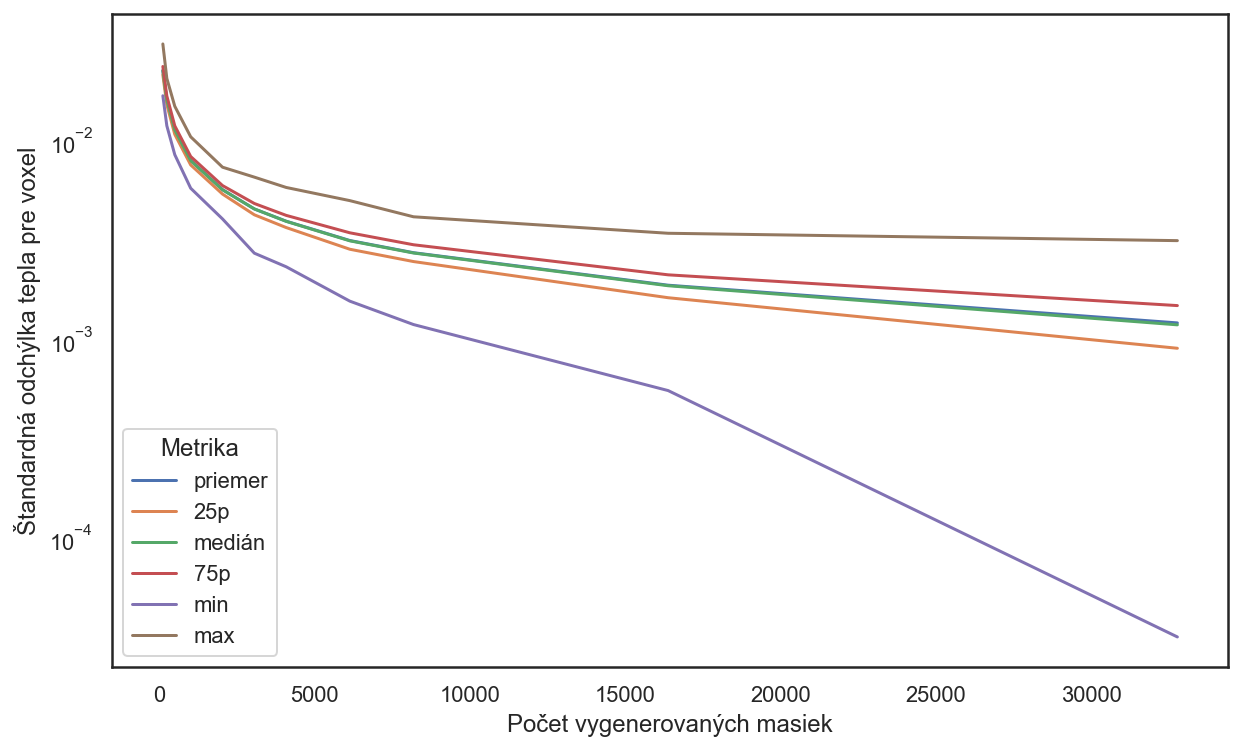
\includegraphics[width=14cm]{assets/images/risei_stability_1.png}
    \caption{Stabilita vytvorených tepelných máp podľa počtu vygenerovaných masiek. Os $y$ je v logaritmickej škále a reprezentuje chybu. Táto chyba klesá logaritmicky s vyšším počtom vygenerovaných masiek. Priemer sa veľmi blíži mediánu, preto ho na diagrame nie je takmer vôbec vidieť.}
    \label{fig:risei_stability_1}
\end{figure}

\subsubsection{Experiment 2 (viacero snímkov)}

Keďže sme v predchádzajúcom experimente overovali stabilitu iba na jednom snímku, v tomto experimente overíme stabilitu na viacero snímkoch. Z testovacej sady sme vybrali 5 TP (viď. \nameref{sec:dictionary}), 5 TN, 5 FP a 5 FN pozorovaní (tj. celkovo 20 pozorovaní), podľa toho ako ich neurónová sieť označila. Takto zabezpečíme vyváženosť tried pozorovaní v experimente. Kvôli časovej aj pamäťovej náročnosti tohto experimentu sme vytvárali 10 tepelných máp pre každé jedno pozorovanie. Výsledky boli takmer identické s predchádzajúcim experimentom (Sekcia \ref{sec:risei_stability_1}) a trend poklesu chyby pri zvyšujúcom počte masiek bol zachovaný (\ref{tab:risei_stability_2}). Z oboch experimentov vyplýva, že je vhodné použiť vyšší počet masiek pri vytváraní tepelných máp, aby sa odstránil vyplyv náhody. Ako vhodným počet považujem 2048 masiek, pri tomto počte je chyba vzhľadom na hodnoty v tejeplnej mape minimálna (Tavuľka \ref{tab:risei_stability_1}, \ref{tab:risei_stability_2}).

\begin{table}[]
    \centering
    \begin{tabular}{|r|r|}
    \hline
    \multicolumn{1}{|c|}{\begin{tabular}[c]{@{}c@{}}Počet vygenerovaných\\ masiek\end{tabular}} &
      \multicolumn{1}{c|}{\begin{tabular}[c]{@{}c@{}}Medián štandardnej\\ odchýlky pre voxel\end{tabular}} \\ \hline
    16   & 0.0594 \\ \hline
    128  & 0.0207 \\ \hline
    256  & 0.0160 \\ \hline
    512  & 0.0105 \\ \hline
    1024 & 0.0074 \\ \hline
    2048 & 0.0052 \\ \hline
    3072 & 0.0043 \\ \hline
    4096 & 0.0037 \\ \hline
    \end{tabular}
    \caption{Stabilita vytvorených tepelných máp podľa počtu vygenerovaných masiek pre 20 snímkov. Trend poklesu chyby oproti prvému experimentu (Tabuľka \ref{tab:risei_stability_1}) ostal zachovaný.}
    \label{tab:risei_stability_2}
\end{table}

\subsection{RISE vs RISEI}

V tomto experimente sme porovnali RISE a rôzne nastavenia metódy RISEI. Použili sme 3D CNN model s úspešnosťou 72\%, senzitivitou 73\% a špecificitou 71\%, toto nie je rovnaký model ako ten, ktorý sme použili v predchádzajúcom experimente, ale jeden z prvých modelov, ktorý sme natrénovali. pretože sme sa snažili overiť metódu RISEI čo najskôr. Najnovší 3D CNN model sme ešte nestihli použiť v tomto experimente. 

Použili sme rovnaké nastavenie parametrov ako v predchádzajúcom experimente (Sekcia \ref{sec:experiment_rise_various_architectures}) a menili sme len parametre \textit{b1}, \textit{b2} a \textit{b2\_value}. Parametre \textit{in\_paint\_radius} sme nastavili na hodnotu $5$. Vyhodnocovali sme zatiaľ len metriku \textit{insertion}, najlepšie výsledky sme dosiahlli bez použitia dokreslenia ale s prekrytím hodnotou jedna (Tabuľka \ref{tab:experiment_risei_various_configuration}). Metóda s dokreslením si počínala horšie, ale stále lepšie ako prekrytie s hodnotou nula pôvodná metóda RISE). Obrázok \ref{fig:heatmap_and_auc_example} zobrazuje príklad vygenerovanej tepelnej mapy pre MRI snímok a výsledný graf zmeny aktivácie pre metriky \textit{insertion}.

\begin{table}[]
    \centering
    \begin{tabular}{l|l|l|}
        \cline{2-3}
                                                                    & \multicolumn{2}{c|}{Insertion} \\ \cline{2-3} 
                                                                    & Priemer        & Medián        \\ \hline
        \multicolumn{1}{|l|}{b1 =  0, b2 = 1, b2\_value = min (RISE)} & 0.43           & 0.37          \\ \hline
        \multicolumn{1}{|l|}{b1 =  0, b2 = 1, b2\_value = max}        & \textbf{0.65}  & \textbf{0.67} \\ \hline
        \multicolumn{1}{|l|}{b1 =  0, b2 = 1, b2\_value = median}     & 0.52           & 0.48          \\ \hline
        \multicolumn{1}{|l|}{b1 =  1, b2 = 0}                        & 0.53           & 0.47          \\ \hline
        \multicolumn{1}{|l|}{b1 =  1, b2 = 0.25, b2\_value = min}     & 0.49           & 0.42          \\ \hline
        \multicolumn{1}{|l|}{b1 =  1, b2 = 0.5, b2\_value = min}      & 0.44           & 0.37          \\ \hline
        \multicolumn{1}{|l|}{b1 =  1, b2 = 0.75, b2\_value = min}     & 0.39           & 0.30          \\ \hline
    \end{tabular}
    \caption{\textbf{Porovnanie rôznych nastavení metódy RISEI.} Najlepšie výsledky dosiahla metóda bez použitia dokreslenia ale s prekrytím hodnotou jedna.}
    \label{tab:experiment_risei_various_configuration}
\end{table}

\begin{figure}[h!]
    \centering
    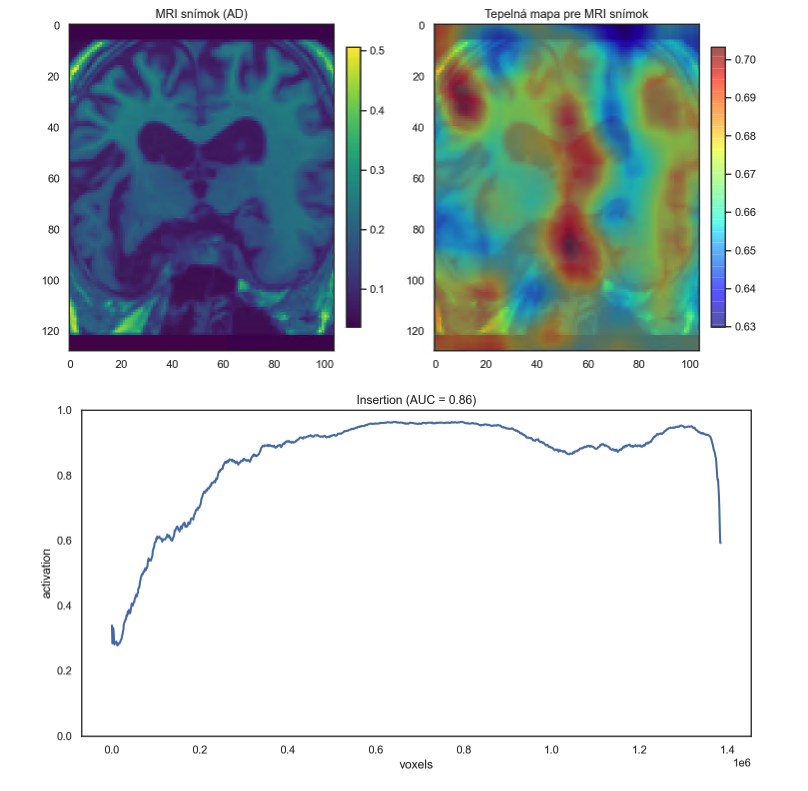
\includegraphics[width=14cm]{assets/images/heatmap_and_auc_example.png}
    \caption{Vygenerovaná tepelná mapa a graf zmeny aktivácie po pridávaní voxelov pre vybraný MRI snímok. Metrika AUC je pomerne vysoká, avšak je potrebné tepelnú mapu ešte vyhodnotiť z pohľadu segmentačných masiek. Tepelná mapa bola vygenerovaná s parametrami \textit{b1 = 1, b2 = 0}.}
    \label{fig:heatmap_and_auc_example}
\end{figure}

Ako možná zmena do ďaľších experimentov je používať hodnotu \textit{max} ako hodnotu pre parameter \textit{b2\_value} v kombinácii s \textit{b1 = 1} (tj. metóda s dokreslením) a \textit{b2 < 1}, keďže dosiahla zatiaľ najlepšie výsledky.

\subsection{Hľadanie optimálnych parametrov}

\subsection{Porovnanie s existujúcimi metódami}

\section{Zhrnutie}

Zistili sme, že metóda RISE s dokresľovaním dosahuje lepšie výsledky ako pôvodná metóda ktorá zakrývala minimálnou hodnotou. Pokial ale minimálnu hodnotu nahradíme maximálnou, dosiahneme lepšie výsledky ako s dokreslovaním, ktoré dosahuje podobné vśyeldky ako zakrývaním mediánom. Avšak, vyhodnocovali sme zatiaľ len pomerne malej vzorke a nebrali sme do úvahy početnosť tried (AD a CN) v tejto vzorke čo je nedostatkom našich experimentov (v ďaľších experimentoch by mali byť tieto triedy vyvážené). Zároveň na dátach z tejto vzorky nemali testované modely 100\%-nú úspešnosť.

Na generovanie tepelných máp sme použili 1000 masiek (keďže autori metódy RISE v experimentoch použili podobný počet), avšak my máme iný typ dát (3D volumetrické dáta), preto je vhodné vyskúšať rôzne počty a nájsť vhodný počet pre náš problém.

Keďže sú masky pri generovaní tepelných máp náhodné, je možné, že pre jeden MRI snímok metóda vygeneruje rôzne tepelné masky. V ďaľších experimentoch by sme mali vyhodnocovať aj konzistenciu tepelných máp - tj. ako veľmi sa líšia medzi rôznymi použitiami metódy na tom istom snímku. Predpokladáme, že väčší počet použitých másk bude viesť ku konzistentnejším tepelným mapám. Takýmto meraním môžeme dospieť k optimálnemu počtu masiek, ktorý je potrebný na generovanie tepelnej mapy.

Taktiež je potrebné vyhodnotiť správnosť tepelných máp vzhľadom na segmentačné masky, tak ako sme uviedli v návrhu riešenia (Sekcia \ref{sec:heat_maps_and_model_segmentation_masks}). Ďalej je potrebné porovnať navrhovanú metódy s inými existujúcimi metódami, napr. LRP alebo analýza senzitivity.


% TODO: we need to compare our method with other methods like LRP or other oclussion methods
% TODO: evaluate the consistency of heatmaps, the method several times for the same image and find out if heatmaps are consistent - this way we can find also optimal number of masks
% TODO: compare with segmentation masks, if more heat is in important areas
